\documentclass[11pt, a4paper]{article}
\usepackage[a4paper, total={6in, 9.5in}]{geometry}

\title{\textbf{\Huge Gravitational Wave Physics and LIGO}}

\usepackage{amsmath, tensor, gensymb, graphicx, hyperref, authblk, amsfonts, amssymb, verbatim, wrapfig, subfig}
\usepackage[T1]{fontenc}
\usepackage[utf8]{inputenc}
\usepackage[english]{babel}
\usepackage[bottom]{footmisc}
\usepackage[sorting = none]{biblatex}

\hypersetup{
    colorlinks=true,
    linkcolor=blue,
    urlcolor=blue,
    citecolor=black}
\urlstyle{same}

\addbibresource{bibliography.bib}

\author[1]{Sagar JC}
\author[1]{Aditya Srivatsa}
\author[1]{Ajith U Shanbhag}
\author[2]{Kushal J}
\author[3]{Hardik Medhi}
\author[4]{Bhavya Goradia}
\author[5]{Kshitija Kshirsagar}
\author[6]{Tasmi Memon}
\author[7]{Samrudhi R Kanjarpane}
\author[8]{Ajay Atwal}
\author[9]{Tanay}
\author[10]{Divyanshi Agrawal}
\author[10]{Kirti Jadhav}
\author[10]{Ved Deshpande}
\author[11]{Dhyan Gandhi}

\affil[1]{St. Joseph's College, Bengaluru}
\affil[2]{Christ Junior College, Bengaluru}
\affil[3]{REVA University, Bengaluru}
\affil[4]{KJ Somaiya College of Engineering, Mumbai}
\affil[5]{Institute of Science, Nagpur}
\affil[6]{Maharaja Sayajirao University, Vadodara}
\affil[7]{Poornaprajna College, Udupi}
\affil[8]{University of Hyderabad, Hyderabad}
\affil[9]{Mumbai University, Mumbai}
\affil[10]{St. Xavier's College, Mumbai}
\affil[11]{Manipal Institute of Technology, Udupi}

\renewcommand\Authands{ and }

\date{\today}

\begin{document}
\maketitle

\section*{Acknowledgement}
\input{Acknowledgement}

\pagebreak
\begin{center}
    \section*{Abstract}
\end{center}

\input{0 Abstract}

\providecommand{\keywords}[1]
{
  \small	
  \textbf{\textit{Keywords---}} #1
}

\keywords{General Relativity, Space time, Tensors, indices, Field equations, Wave equation, Polarization, Energy Flux, Doppler effect, Inverse square law, Inspiral mechanism, Black holes, Neutron stars, Pulsars, Revolving Binary system, LIGO, Interference, Coherency, Laser}
\pagebreak

\tableofcontents
\pagebreak

\section{Introduction}
\input{1 Introduction}

\section{Linearized theory of Gravitational waves}
\input{2 Linearized_theory}

\section{Properties of Gravitational waves}
In this section we shall know about the properties of gravitational waves. Gravitational waves can be characterised by its frequency, amplitude, period. The propagate with the same speed of Electromagnetic waves. Unlike Electromagnetic waves, the wavelength of GW’s can range from a kilometer to the size of the universe itself. Since the wavelength of gravitational waves is larger than the source, they cannot be used for imaging. In contrast to electromagnetic waves which are polarised at 90 degree, i.e orthogonal plane polarized EM waves have their plane 90 degrees apart, where as for gravitational waves it is at 45 degree which will be discussed in the next session. GWs do not interact with matter, but electromagnetic waves do. Electromagnetic waves are known to exhibit a wave-particle duality nature unlike Gravitational waves, the nature of which is still unknown. Although there are quite a few similarities between these two, gravitational waves open a new different window to view the universe. \cite{Thorne:1995xs}

\begin{figure}[h]
    \centering
    \includegraphics[height= 7cm, width=9cm]{images.tex/GW_propagation.jpg}
    \caption{Propagation of GW wave. Source :- \href{https://www.einstein-online.info/en/spotlights/gravwav/gravwav-sub01/}{Einstein-online.info}}
\end{figure}

\begin{figure}[h]
    \centering
    \includegraphics[height= 8.7cm, width=12cm]{images.tex/EM_propagation.png}
    \caption{Propagation of EM wave. Source :-\; \href{https://www.toppr.com/guides/physics/communication-systems/propagation-of-electromagnetic-waves/}{Topper.com}}
\end{figure}

\pagebreak

\subsection{Polarization of Gravitational waves}


Gravitational waves can also be. Since they are three dimensional waves their polarization can be restricted to two forms where the the amplitude tensor $A^{\mu\nu}$ has two forms $A^{\mu\nu}_{+}$ and $A^{\mu\nu}_{\times}$ which are orthogonal to each other \cite{Dirkes_2018}. They can be represented as 

\begin{equation}
    A^{\mu\nu}_{+} = h_{+}\, \varepsilon^{\mu\nu}_{+}
\end{equation}

\begin{equation}
    A^{\mu\nu}_{\times} = h_{\times} \,\varepsilon^{\mu\nu}_{\times}
\end{equation}

\noindent where $\varepsilon^{\mu\nu}_{+}$ and $\varepsilon^{\mu\nu}_{\times}$ are unit polarization tensors.

\begin{equation}
\varepsilon^{\mu\nu}_{+} =
\begin{bmatrix}
0 & 0 & 0 & 0 \\
0 & +1 & 0 & 0 \\
0 & 0 & -1 & 0 \\
0 & 0 & 0 & 0 \\
\end{bmatrix}
\end{equation}
\\
\begin{equation}
\varepsilon^{\mu\nu}_{\times} =
\begin{bmatrix}
0 & 0 & 0 & 0 \\
0 & 0 & +1 & 0 \\
0 & +1 & 0 & 0 \\
0 & 0 & 0 & 0 \\
\end{bmatrix}
\end{equation}

\noindent In general relativity any tensor with indices $\mu\nu$ is a rank 2 tensor with 4 rows and 4 columns where each index can take values of space time coordinates which are $(t,x,y,z)$ , and position of each element is associated with any two coordinates. Thus in such tensors, the positions of elements are associated with space-time as follows:

\begin{equation*}
\mu\nu =
    \begin{bmatrix}
    tt & tx & ty & tz \\
    xt & xx & xy & xz \\
    yt & yx & yy & yz \\
    zt & zx & zy & zz \\
    \end{bmatrix}
\end{equation*}

\noindent So when we compare the unit polarization tensors $\varepsilon^{\mu\nu}_{+}$ and $\varepsilon^{\mu\nu}_{\times}$ with the above one, we see that in $\varepsilon^{\mu\nu}_{+}$ the non zero entries are +1 in $`xx$' direction and -1 in $`yy$' direction, hence the $A^{\mu\nu}_{+}$ amplitude is oriented only along X and Y axes, thus this gravitational wave which oscillates along X and Y axes is called as `PLUS' polarized wave because the vibration resembles `+' symbol. But in $\varepsilon^{\mu\nu}_{\times}$ the non zero entries are +1 in $`xy$' direction and -1 in $`yx$' direction, hence the $A^{\mu\nu}_{+}$ amplitude is oriented in the `XY' plane at a an angle of 45$\degree$ to the axes, thus this gravitational wave which oscillates in the `XY' plane at a an angle of 45$\degree$ to the axes is called as `CROSS' polarized wave because the vibration resembles `$\times$' symbol. So the equation of polarized gravitational waves are:-\\

\hspace{0.7cm} (+) wave $\Rightarrow $  $\tilde{h}_{\mu\nu} = h_{+}\, \varepsilon^{\mu\nu}_{+}\, e^{i(\omega t - k_{z}z)}$ \hspace{2mm} and \hspace{2mm} $(\times)$ wave $\Rightarrow $  $\tilde{h}_{\mu\nu} = h_{\times}\, \varepsilon^{\mu\nu}_{\times}\, e^{i(\omega t - k_{z}z)}$
\\

\noindent Here the position variable is just `$z$', assuming that the wave is travelling along z axis and space-time is oscillating in the X-Y plane, which helps us to visualize polarized GWs easily.

\begin{figure}[h]
    \centering
    \includegraphics[height=4.3cm, width = 9.5cm]{images.tex/polarization_simulation.jpeg}
    \caption{Simulation of Polarized waves. Source:- \href{https://sudonull.com/post/7567-Einstein-Telescope-a-new-generation-gravitational-wave-detector}{Sudonull.com}}
\end{figure}

\pagebreak
 
\input{3 Properties.tex/3.2 Effect of gw on object}
\input{3 Properties.tex/3.3 Energy transported}

\section{Sources of Gravitational waves}
\input{4 Source.tex/4.0 source_intro} 
\input{4 Source.tex/4.1 Single accelerating object}
\input{4 Source.tex/4.2 Revolving binary system}
\input{4 Source.tex/4.3 Neutron star collission}
\input{4 Source.tex/4.4 PBH}

\section{Types of Gravitational Waves}
\hspace{0.6 cm} Gravitational waves are produced by each and every body which is accelerating, for e.g. moving cars, air planes, humans, etc. However, they are too small to be noticed and detected with our current technology. In order to study gravitational waves, we need to look at object which are massive and much more bigger than our own solar system like black holes, neutron stars, or huge stars at the end of their lives like gamma ray bursts, pulsars, orbiting black holes, rapidly spinning neutron stars, etc. In fact our universe is filled with many such objects which produce gravitational waves with a significant amplitude and energy. This section was referred by \cite{Linear}, \cite{Allen1996TheSG}, \cite{Neutron_wiki} , \cite{sounds_of_space} \\

\noindent Gravitational wave sources have been divided into following categories:-

\begin{enumerate}
    \item \textbf{Short duration sources :-} Compact binary coalescence, supernovae, gamma ray burst.

    \item \textbf{Continuous sources :-} Pulsars, magnetars, rapidly spinning neutron stars, low mass X Ray binaries, super massive black hole binaries.

    \item \textbf{Stochastic sources :-} Metric fluctuations generated in the very early universe.
\end{enumerate}

\noindent To understand gravitational waves better, LIGO scientists have divided the waves in four categories. The division of the gravitational waves is based on their sources and their characteristic vibration as detected by the interferometers.  They are divided into Continuous, Compact Binary Inspiral, Stochastic and Burst Gravitational waves.

\begin{enumerate}

\item \textbf{Continuous Gravitational Waves} 
    
\noindent Such Gravitational Waves are produced by objects that have constant frequencies and amplitude like a single spinning neutron star. Neutron stars are basically a result of the supernova explosion of a massive star, combined with gravitational collapse, that compresses the core so much that the star density becomes as that of atomic nuclei. Radius of neutron stars will be in the order of 10 kilometers, and mass will be around 1.4 Solar masses. So density will be around $10^{17}\: \text{Kg}\text{m}^{-3}$. The properties of the gravitational waves depend on the spin rate of the star. Therefore, if the spin rate is constant, the properties of gravitational waves (frequency and amplitude) will also remain constant i.e. \textit{continuous}. Spinning neutron stars that possess asymmetric deformations or imperfections in their space produce gravitational waves as it swiftly rotates about its axis. The reasons or effects which can produce asymmetry could be Accretion (large mountain), Magnetic deformations or Pulsar glitches.

\vspace{0.2cm}

\item \textbf{Compact Binary Inspiral Gravitational Waves}
    
\noindent Most of the waves detected so far by LIGO are part of this category. Compact Binary In spiral Gravitational Waves are formed by orbiting pairs of massive objects like neutron stars or black holes. There are three kinds of systems in this category of gravitational wave generators where each one has different characteristics. They are Binary Black Hole system (BBH), Binary Neutron Star system (BNS) and Black Hole-Neutron Star binary system (BHNS). The main phases involved in such systems are spiral, merger and ring-down.

\vspace{1mm}
Let us start by considering two black holes orbiting each other. Initially they are widely separated, spiral occurs over millennia, with each revolution, they emit very weak gravitational waves. Slowly as the energy is lost from the system in the form of gravitational waves, the binary is thus pushed into an orbit with smaller radius and higher orbital frequency. Thus the distance between them decreases and their speeds increase. This causes the frequency of the gravitational waves to increase. Now comes the Merger stage where the black holes come very close and are about to collide to form a single black hole and the black hole thus formed has large distortions in its shape. The strongest gravitational waves are emitted during this process. The distortions thus formed are radiated away as more gravitational waves during the ring-down phase and an undistorted but rotating black hole is left behind. Due to the increase in frequency, the pitch also increases and as a result these gravitational waves would produce a chirp sound. Current results indicate that compact binary objects may well be the most promising sources of gravitational waves rather than supernova collapse.

\item \textbf{Stochastic Gravitational Waves}

These types of waves are generated from random sources, typically arising from a large number of unresolved and uncorrelated events and thus they are the most difficult gravitational waves to detect. Stochastic Gravitational Waves are believed to be the result of processes that took place shortly after the big bang. Just like the Cosmic Micro-wave Background (CMB), these gravitational waves arise from a large number of independent, random events merging to create a cosmic gravitational wave background. Due to their random motion, these waves are the most smallest, that's why the final signal has stochastic nature and the difficult to detect with our current technology. These waves may be analyzed statistically but they cannot be predicted precisely. Detecting these gravitational waves from the Big Bang could allow us to see back in the history of the Universe.

\vspace{0.2cm}

\item \textbf{Burst Gravitational Waves}   

Of all the types of gravitational waves, these waves come from the sources which are yet to be known and thus the form of waves which will be produced is also unexpected. Burst gravitational waves come from short-duration unknown sources. Since we are unfamiliar with these sources, thus its modelling is a big challenge since these will not have well defined properties which are known earlier to us like those of compact binary inspiral waves. Some believe that these waves are produced from systems like supernovae. They are believed to have a 'pop' and 'crack' sound. However, it is difficult to say anything as of now due to the lack of knowledge about their origin. But if we discover an efficient way to detect such GW, revolutionary information about the universe could be revealed.

\end{enumerate}

\begin{figure}[h]
    \centering
    \includegraphics[scale=0.6]{images.tex/Stochastic_gw.jpg}
    \caption{Gravitational Wave Spectrum. Source :- \href{https://link.springer.com/article/10.1007/s41114-017-0004-1}{Detection methods for stochastic gravitational-wave backgrounds by Joseph D. Romano}}
\end{figure}

\begin{figure}[h]
    \centering
    \includegraphics[height = 3.5 cm, width = 10cm]{images.tex/Stochastic wave form.jpg}
    \caption{Stochastic gravitational wave form.\, Source :- \href{https://journals.aps.org/prd/abstract/10.1103/PhysRevD.91.022003}{Searching for stochastic gravitational waves using data from the two co-located LIGO Hanford detectors by J. Aasi}}
\end{figure}

\pagebreak


\section{Why study Gravitational Waves}
\hspace{1cm}Gravitational waves are already used as an important member of multi-messenger astronomy and these can be used to study in depth many objects or phenomena such as:

\begin{itemize}

\item Cataclysmic variables
\item Binary Neutron Stars
\item Young Neutron Stars (the r-mode instability)
\item Low-mass X-ray binaries
\item CMB and Galaxy formation

\end{itemize}

\hspace{1cm}Gravitational waves are emitted by the masses and sent as ripples across spacetime which is completely different from the mechanism of production and transmission of EM waves. Therefore, it could give us more information on the subject matter at hand.

\hspace{1cm}Gravitational waves provide further information about black holes that would otherwise be invisible. Gravitational waves also weakly interact with matter (apart from lensing), thereby reducing energy lost or scattered before reaching the detector. This implies better understanding of inconspicuous regions of space, like the interior of a supernova or the Big Bang.

\subsection*{Uses of their Detection}

\hspace{1cm} Gravitational Waves are also used in Astronomy because it allows us to observe the universe the universe in a different way, providing us information about matter such as:\\

\begin{enumerate}
    \item Information about the big bang 
    
    \hspace{1cm}Gravitational waves have travelled almost unimpeded through the universe since they were generated (which happened $10^{-24}$s after the Big Bang, far earlier than the CMB radiation). Possibilities of non-inflation mechanisms that produce gravitational waves are high. One such possibility could be cosmic strings, which ought to be detectable using gravitational waves. Observations of compact binaries in spiral made by the LIGO/VIRGO experiments can to give us a lot more information about the system than just the binary masses and spins.\\
    

    \item Test the theory of General Relativity
    
    \hspace{1cm}They can be used for high-precision tests of general relativity. Radiation reaction to some scalar waves in scalar-tensor theories has a signature that can be found with high precision in LIGO/VIRGO.\\
    

    \item Detection of the Hubble constant
    
    \hspace{1cm}They can be used to measure the Universe’s Hubble constant, deceleration parameter, and cosmological constant.Gravitational waves bring a new window to validate the general theory of relativity and cosmological constant as the perfect/correct theory of gravity and the expanding universe(cosmic acceleration). Hubble's Constant shows the expansion of the Universe by showing how distant galaxies are moving away from us and is given by:
    \begin{equation}
        v = H_0 \times d
        \end{equation}
        
        where, v is the Velocity of a galaxy, in $kms^{-1}$
        
              $H_{0}$ is the Hubble Constant, measured in $kms^{-1}Mpc^{-1}$
              
              d is the distance of the galaxy from the earth in megaparsecs(Mpc)
        
        \vspace{1cm}
        
        \begin{figure}[h]
            \centering
            \includegraphics[scale=0.9]{images.tex/HCGW.jpg}
            \caption{Hubble's Constant using Gravitational waves.\\
            Source :- \href{https://www.researchgate.net/profile/Michael-Ross-9/publication/324600496}{A gravitational-wave standard siren measurement of the Hubble constant, Pg 3}}
        \end{figure}

    \item Polarization of Gravitational waves
    
    \hspace{1cm}Gravitational waves carry 2 independent polarizations. A wave will usually have a combination of both. Some sources (rotating) will emit both polarizations with some lag between them. Studying this would give the nature of the source and its rotation.\\

    \item Centrifuge of Binary Stars
    
    \hspace{1cm}A more careful calculation shows that, for unequal masses, the quadrupole amplitude and the rate of shrinking depend on the masses only through the combination:
    \begin{equation}
    \ M=\mu^{3/5} \times M^{2/5}\
    \end{equation}
    \hspace{1cm}This is called the chirp mass, where, $\mu$ is the reduced mass and M the total mass. The chirp mass can be easily determined if the shrinking time is observed in gravitational radiation. After measuring the amplitude, the only quantity that would not be known to us is the radial distance r from here to the source. By observing the gravitational waves that are produced by shrinking orbits due to loss in energy via gravitational radiation, we can thus obtain the distance to the source. This is another example how gravitational wave observations provide information that is hard to find using electromagnetic waves.\\

    \item Spiralling of Black Holes and Neutron Stars
    
    \hspace{1cm}For a Neutron star or black hole spiralling inwards, the inward spiral has a sort of “map” of it that are emitted in the form of gravitational waves. Analysis of these waves could give information of the body, help determine the type of body(black hole or any other exotic object like a naked singularity)  and can be studied better by LISA for low masses and high frequencies as opposed to LIGO/VIRGO that can capture large masses and low frequencies.\\
    

    \hspace{1cm}Conclusively, we can say gravitational waves provide a new tool for astronomy as well as cosmology and will be ever evolving in terms of types of observations possible ranging from new ways to test for dark matter and the validity general relativity with high precision and observations that simply would not be possible with just electromagnetic waves.This also provides an alternate method to validate the cosmological constant, Hubble’s constant, and various other uses. This section was referred from these papers \cite{Schutz_1999},\cite{Mukherjee_2020}.

\end{enumerate}

\pagebreak


\section{Indirect Evidences of Gravitational Waves}
\hspace{0.6cm}Neutron stars are highly compacted core of a dead star, left behind as a remnant of supernova explosion. The pulsars are a unique type of neutron stars that emits beams of electromagnetic radiation out of its magnetic poles. The radiation can be detected from the Earth as blinking star through radio telescopes. The radiation is emitted in the periodic pattern so it appears as a pulsed emission of radiation. The discovery of pulsars was done by Jocelyin Bell a graduate student at Cambridge University in England in the year 1967 who was working under Antony Hewish \cite{AstronomyAndbeyond:1999}. She found out a peculiar pattern in the data in the form of regular pulses. This data was different from the radio signals of the celestial bodies that they detected earlier. At first, they thought that the signal is from some alien civilization so they named them as Little Green Men (LGM) but after few weeks they observed that there were three more objects in the other parts of the sky pulsing with different periods hence they dropped the name Little Green Men and renamed them as Pulsar.\\

Pulsars are among the strangest objects within the universe. Astronomers and scientists use pulsars as an instrument to detect gravitational waves. Pulsars are still found by using large radio telescopes. The largest radio telescope in the world is located at Arecibo in Puerto Rico. A telescope scans the entire sky and scientists look for objects that appear in and out. When a pulsar rotates, it produces detectable pattern of radio emission which is very precise and repeats periodically. Its maximum intensity rises and falls every 23 hours 56 minutes. Pulsars spin because the stars from which they are formed also rotate. The slowest pulsar ever detected spins on the order of one per second and the fastest pulsars can spin hundreds of times per second from earth, pulsars often look like flickering stars. On and off, on and off and they seem to blink with a regular rhythm. But the light waves from pulsars doesn't actually flicker or pulse. It radiates two steady, narrow beams of light in opposite direction. The light from the beam is steady and pulsars appear to flicker because they also spin for the same time. \cite{AstronomyAndbeyond:1999}\\

Pulsars are considered to be a great tool in determining the existence of gravitational waves.In 1974 the first evidence of gravitational waves was deduced through the motion of the double neutron star system PSRB1913+16  \cite{Linear}. In this system one of the star is a pulsar which emits electromagnetic pulses at radio frequencies precisely at regular intervals as it rotates. Russell Hulse and Joseph Taylor discovered this binary pulsars also noticed that the frequency of pulses shortened and the stars were gradually spiraling towards each other with an energy loss which is closely equal to the energy predicted to be radiated by gravitational waves. For this discovery, Hulse and Taylor were awarded the Nobel Prize in Physics 1993 \cite{Lommen_2015}. Further observations of the binary pulsar and other multiple systems also agree with the General theory of Relativity to high precision. This evidence of gravitational waves is considered as the first indirect evidence of gravitational waves. 
 
\begin{figure}[h]
    \centering
    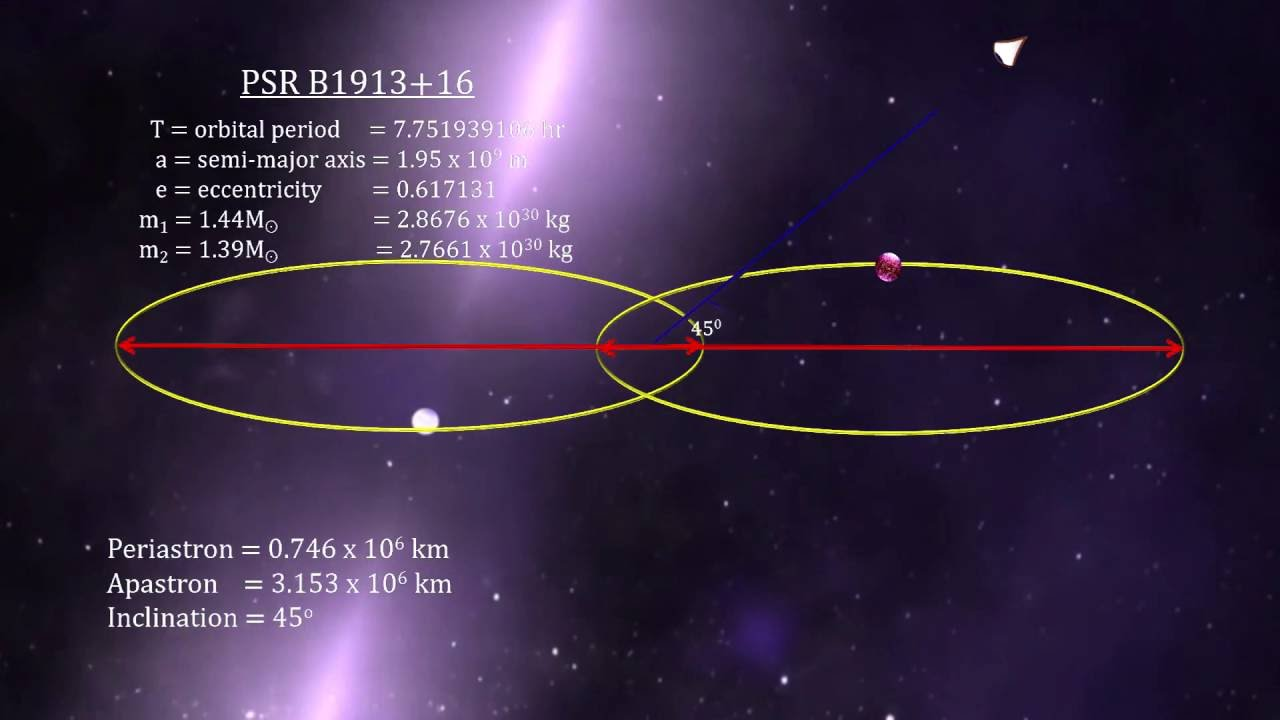
\includegraphics[scale=0.255]{images.tex/PSR-B191316.jpg}
    \caption{Binary pulsar PSR B1913+16. Source :- \href{https://www.astroblogs.nl/wp-content/uploads/2014/03/PSR-B191316.jpg}{Astroblogs.nl}}
\end{figure}

\pagebreak


\section{Direct search for Gravitational waves}
A successful attempt to detect gravitational waves was made by LIGO. It stands for Laser Interferometer Gravitational wave Observatory), and was founded by Reiner Weiss (MIT) , Barry Barish (Caltech) and Kip Thorne (Caltech). A joint - initiative to establish LIGO was taken by MIT and Caltech, and was funded by the National Science Foundation(NSF). The construction of the two detection sites at remote locations of Hanford and Livingston, commenced in 1994 and ended in 1999. \\

Two sites were built instead of one, in order to avoid detection of an anomaly caused by external events of the particular location. In addition to the detection sites, LIGO also includes two primary university research centers; MIT and Caltech. The Initial LIGO project, which used the very first interferometers built for observations, was conducted from 2002 to 2010. During this period, not a single detection was made. Later on, an upgraded version of the same, The Advanced LIGO project was installed over the span of four years, between 2010 to 2014. Within days of initiating observations with newly installed equipment, LIGO made the first successful detection of gravitational waves on September 14, 2015. The gravitational waves detected, were known to have originated from the collision of two black holes in a binary system, which is 1.3 billion years away. Seeing it’s success over years, the co-founders were awarded a Nobel Prize in the year 2017.

Currently, LIGO employs around 40 people for each construction site. They are engineers, technicians and scientists who operate and overlook the functioning of the instruments and systems. On the other hand, LIGO engineers at Caltech and MIT work on improving LIGO’s stability and sensitivity, and the LIGO physicists and astrophysicists interpret the nature of the detected gravitational waves. LIGO’s mission is to open a window for a new area of scientific research on gravitational-wave astrophysics. It also conducts public outreach programs in order to provide opportunities for the scientific community to contribute to the enhancement of detectors, observation and data analysis. 


\subsection{Principle of LIGO}

When the gravitational wave reach us, without a doubt, they are only very weak perturbations on our local flat space. Be that as it may, they will provide information about the strong-field regions where they began. it will additionally permit us to decide the wave properties of the gravitational radiation—for ex-sufficient, their spread speed and polarization states \cite{barish1999ligo}. The essential construction of LIGO's interferometers differs a little from the interferometer that Michelson planned more than 125 years prior, however for certain additional highlights. The visible pattern occurring where the coherent waves intersect is simply an "interference" pattern.\cite{collaboration2015advanced}

\subsubsection{Interference Pattern}

In  nature,  the  peaks  and  troughs  of  one  wave cannot absolutely  meet  the  peaks or  troughs  of  another  wave. Regardless  of  how in-sync they are once they merge, the peak of the wave coming out from the interference always equals the sum of the heights of the merging waves on every point wherever they are physically interacting. What  dictates how  well-aligned  the  beams are once  they  merge  is  the path length  they travel before merging. So the core principle of LIGO is interference of light. When the path difference between two light wave is equal to integral multiple of wavelength, then constructive interference occurs where the resultant light will have maximum brightness. And if the path difference is equal to half-integral multiple of wavelength, then destructive interference occurs and resultant light will have minimum brightness. \\

If the beams travel precisely the same distance, their light waves will be absolutely aligned such that they lead to total destructive interference (LIGO is designed to get total destructive interference if no gravitational waves are detected).  But if the lasers don’t travel identical distances, their light waves are not any longer in synchronize as they merge, which implies no light, a bit light, or a light as bright because the original laser beam reaches the photodetector.  And if the arms are changing length over time, a flicker appears as the beams suffer a variety of interference. This time difference is manifested within the interference pattern once the two laser beams superimpose on the path to the photodetector, which can quantify stage movements to ten-billionths of an interference fringe.\cite{barish1999ligo}\\

\begin{figure}[htpb]
    \centering
    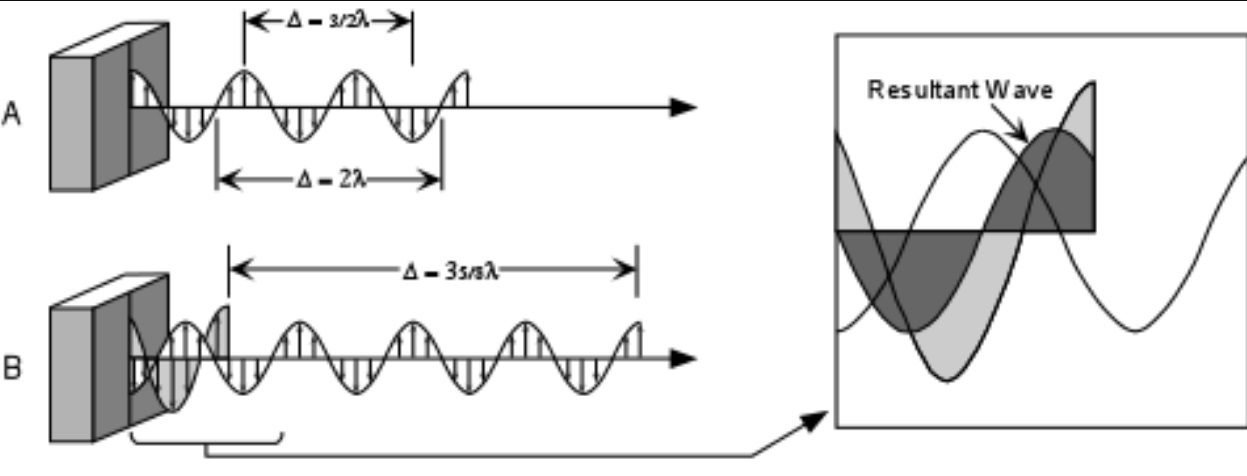
\includegraphics[scale=0.585]{images.tex/interference.jpg}
    \caption{Interference. Source :- \href{https://www.tulane.edu/~sanelson/eens211/interference_of_light.htm}{Interference Phenomena by Prof. Stephen A. Nelson}}
\end{figure}

\subsubsection{Differential mode of vibration}

The gravitational waves result in the space to stretch in a direction, at the same time,  compress in a direction perpendicular to it. In LIGO, this results in one arm getting longer whereas the opposite gets shorter, then the other way around, back and forth as long because the wave is passing.  The technical term for this motion is “Differential Arm” motion, or differential displacement, since the arms are at the same time are differing in lengths in opposing ways in which, or deferentially. So because the lengths of the arms differ, thus too will the total path traveled by every laser beam.

\begin{figure}[h]
    \centering
    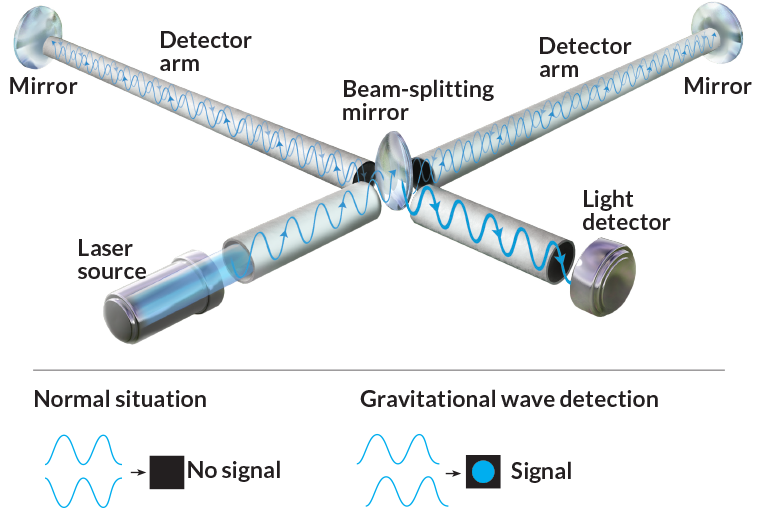
\includegraphics[scale=0.52]{images.tex/Interferometer.jpg}
    \caption{Michelson interferometer.\; Source :- \href{https://www.sciencenews.org/article/trio-wins-physics-nobel-prize-gravitational-wave-detection}{Sciencenews.org}}
\end{figure}

So because the lengths of the arms change, so too does the space traveled by each beam . A beam travelling in the shorter arm will return to the beam splitter before the beam which is ravelling in the extended arm, then things switches because the arms oscillate between being longer and shorter. Arriving at different times, then the LASER does not meet nicely when recombined at the beam splitter. Instead, they shift in and out of alignment or "phase" as they merge. Unlike optical or radio telescopes, LIGO doesn't see electromagnetic waves. It doesn't need to because gravitational waves aren't a part of the spectrum. In fact, electromagnetic wave is so unimportant to LIGO that its detector components are completely isolated and sheltered from the surface world.

\pagebreak

\subsection{Construction of LIGO}

\hspace{1cm} The idea of a laser interferometer to detect LIGO started in the 1960s, where American scientists like Joseph Weber, Soviet scientists Mikhail Gertsenshtein and Vladislav Pustovoit, merged their ideas of a basic interferometer based on Michelson's interferometer. In 1967, Rainer Weiss affiliated to Massachusetts Institute of Technology (MIT) published his paper on the analysis of usage of interferometer and with the help of military funding he initiated the construction of interferometer prototype, but it couldn't be completed. But in 1968, Kip S. Thorne did extensive research on gravitational waves and their sources at Caltech, then he was convinced that interferometers could successfully detect gravitational wave. Thus finally LIGO was constructed in Hanford, Washington in 1994 and Livingston, Louisiana in 1995. The construction was completed by 1997, under Barish's leadership.  After successful detection of GW150914, in 2017, Rainer Weiss, Kip Thorne and Barry C. Barish who were the frontiers of Gravitational wave detection won the Nobel Prize in Physics. \\
LIGO is constructed in such a way that it can even feel the changes in the weakest fundamental force. Some important parts of this Gigantic detector are:- 

\subsubsection{LIGO arms}

LIGO's arms are placed orthogonal to each other which extends for $4\,km$ into two perpendicular directions. The arms of LIGO are made of cylindrical tubes each $20\,m$ in length, welded together whose diameter is $1.2\,m$. The tube is made of 304L-steel with a thickness of $3\,mm$ \cite{carpenter2000laser}. This particular material has extremely low carbon content making it relatively resistant to corrosion when compared to other. The tubes are evacuated to a pressure of $10^-10 to 10^-8 torr.$ This is to prevent the scattering of laser and also to not allow sound to interfere (as sound cant travel in vacuum). The arm is constantly evacuated by the Ion pumps to maintain the vacuum inside the arms. Initially when LIGO was set-up it took approximately 40 day to fully evacuate the beam tubes, and it was heated to 150\degree C to remove residual gases. \cite{vacuum} 

\begin{figure}[h]
    \centering
    \subfloat[]{\includegraphics[width = 7 cm, height = 5 cm]{images.tex/BEAM_TUBE_SEGMENT.png}}
    \qquad
    \subfloat[]{\includegraphics[width = 7 cm, height = 5 cm]{images.tex/C.S view of ligo arm.jpg}}
    \caption{(a) LIGO Beam tube. Source :- \cite{vacuum} (b) C.S view of beam tube. Source:- \cite{althouse2001precision}}
\end{figure}

\subsubsection{Laser system}

The laser used in LIGO has active material to be Nd-YAG (Neodymium - Yttrium Aluminium Garnet) and diode as the pump. Initially the laser output is $4\,W$ and wavelength of lasing light is $808\,nm$ wheich is in near infrared range. This light travels through Non-Planar Ring Oscillator (NPRO), from which a $2\,W$, $1064\,nm$ light called seed beam is generated. This is the laser which will be amplified and begins it's journey in LIGO interferometer. The seed beam is then passed through a Master-Oscillator Power Amplifier (MOPA), which consists of four thin rods of $3\,mm$ thick and $5\,cm$ long which is made similar to glass, using Nd, Y, Li and F$^{-}$. The laser power increases in each of these four rods and finally a 35W laser with the constant wavelength of 1064nm is obtained. It is now further amplified in a High-Power Oscillator (HPO) which is similar to MOPA. This results in an immensely powerful light of 200W. \cite{laser} 

\begin{figure}[h]
    \centering
    \subfloat[]{\includegraphics[width = 4.5 cm, height = 5 cm]{images.tex/NPRO.jpg}}
    \qquad
    \subfloat[]{\includegraphics[width = 8.5 cm, height = 5 cm]{images.tex/Laser amplification.jpg}}
    \caption{(a) NPRO crystal. (b) schematic representation of laser amplification. \cite{laser}}
\end{figure}


\subsubsection{Beam Splitter and Mirrors}

Each arm carries two fully reflecting mirrors at its ends and a partially reflecting mirror called as Beam splitter is present at the common vertex of the arms. The space between the mirrors forms Fabry-Perot cavity. The light travels 4$km$ from one end to other, but this cavity makes the laser light to reflect approximately 300 times, so apparently the laser travels a total of $1200\,km$, this increases the laser power to $750\, kW$. The mirrors are coated extensively to nanometer smoothness (i.e the imperfections on the surface of mirror is in the order of nanometers). This is required to make the system so precise to detect even very feeble GWs. \cite{mirrors}

\begin{figure}[h]
    \centering
    \subfloat[]{\includegraphics[width = 7 cm, height = 5 cm]{images.tex/LIGO_mirror.jpeg}}
    \qquad
    \subfloat[]{\includegraphics[width = 7 cm, height = 5 cm]{images.tex/Beam splitter.jpg}}
    \caption{(a) Fully reflecting mirror. (b) Beam splitter. \cite{mirrors}}
\end{figure}


\subsubsection{Test mass and Photo-detector}

The fully reflecting mirrors are $40 \,kg$ each with thickness of $20\,cm$ and width of $34\,cm$. They act as test masses and are at 4 kilometers away from each other. This test mass is one among three other mass which are hung to a quadruple suspension system aided by silica fibers. They reduce the effect of noise vibration by 100 million times by the time it reaches the mirrors. This acts as a passive seismic isolation system. \cite{mirrors} Then finally the last component is the photo detector. Since the wavelength of operational laser is $1064\,\nm$, which lies in infrared spectrum, the photo detector should work in the infrared region. LIGO uses Broad Band Photo Detector (BBPD) which is built around a low capacitive, series resistant silicon photo-diode "FFD-100", and coupled to a $50\,\Omega$  Radio frequency amplifier called Teledyne Cougar AP389. \cite{BBPD}

\pagebreak

\input{8 LIGO.tex/8.3 Working}
\subsection{Noise and it's Cancellation by LIGO}

Any disturbance in the surrounding could potentially act as noise for LIGO which tends to interfere with the detector and could produce it's own signal instead of a gravitational wave. So changes in environment like vibrations in earth's crust, movement of vehicles, tides, winds, volcanic eruption, mining, etc. Even intensive changes like Temperature. And even the limitations of systems can add it's own noise to the signal. So broadly noise can be classified into:

\begin{itemize}
    \item Seismic Noise
    \item Thermal Noise
    \item Optical Noise
\end{itemize}

\subsubsection{Seismic Noise}

A gravitational wave is measured by monitoring the relative distance between two test mass surfaces. Any force affecting the centre of mass would then result in an ambiguous and faulty measurement. A ground-based interferometer is mechanically coupled to the earth and the masses are prone to seismically driven vibrations. The dominant part of the seismic power spectrum is at low frequencies. A moderately quiet site will have a spectrum of roughly,

\begin{equation}
    x(f) = \frac{1}{f^2} \times 10^{-8}m(Hz)^{3/2}
\end{equation}

where $x(f)$ is Band-width of the noise as a function of frequency($f$).


\subsubsection*{Passive technique of seismic noise reduction} 
    
It utilizes the inertial response of a mass on a spring. Passive isolation takes advantage of the fact that above the resonant frequency, $f_0$, of the mass-spring system, the response of the mass to driving forces decreases by $(\frac{f_0}{f})^2$ . Systems with lower resonant frequencies give higher isolation at a given frequency. These passive systems can also be staged by suspending one isolation system from the isolated stage of a previous system. The total isolation then is the product of each mass-spring system, $(\frac{f_0}{f})^{2n}$, where `$n$' is the number of stages (assuming the same resonant frequency).
    
\subsubsection*{Active technique of seismic noise reduction}
    
Active isolation techniques employ a bootstrapping method. A proof mass is placed on the platform being isolated. The proof mass is more inertial than the platform it sits on. Monitoring the relative displacement, velocity, or acceleration between the platform and the proof mass generates an error signal when the platform has suffered a disturbance to its state. Feedback control systems are used to correct the error signal, locking the position of the platform to the inertial reference of the proof mass. The level of isolation is proportional to the closed-loop gain of the system when the sensor noise is low enough. The limits to the closed-loop gain, the isolation are the sensor’s bandwidth and noise. An advantage to arranging the isolation system in stages is that loop gain in each stage can be more modest, which is sometimes forced by the available bandwidths and mechanical resonances of the structure.\\

LIGO I uses a simple, multi-layer passive isolation system which places a “wall” in the seismic noise spectrum at roughly 40 $Hz$. The proposed LIGO II seismic isolation is largely active \cite{giaime2000active}. A quiet hydraulic system is used externally to the vacuum chambers which house the test masses. This external system has large dynamic range, and is used primarily to take-out long-time scale drifts and disturbances. A two-stage active isolation system inside the test mass chambers is supported by the external system through bellows. The active system isolates an optical table in all six degrees of freedom, from which the test mass is hung as the lower mass of a quadruple pendulum. This design is expected to move the seismic wall to $ \sim 10 Hz$


\begin{figure}[h]
    \centering
    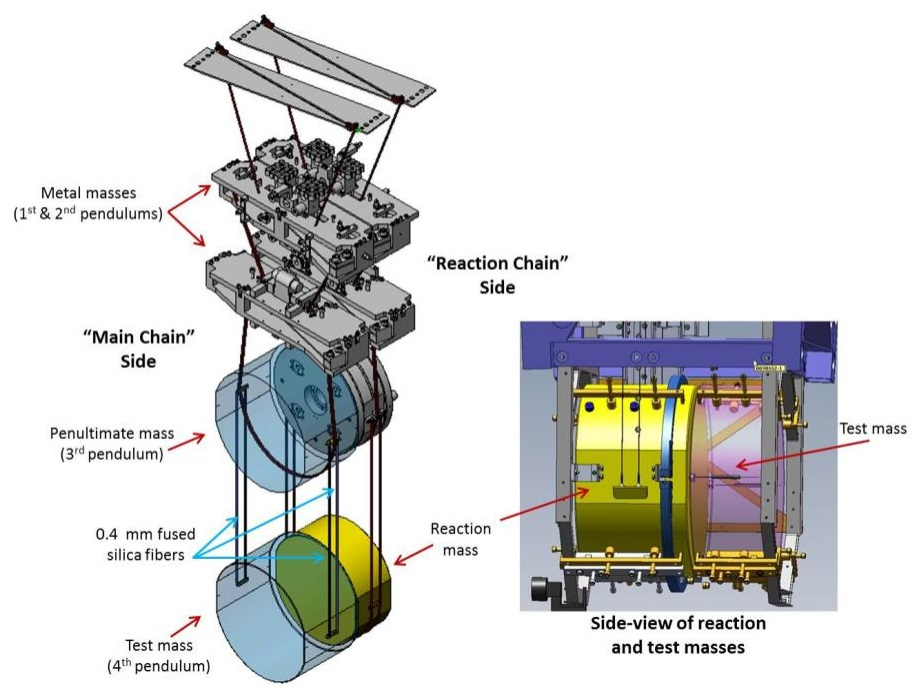
\includegraphics[scale = 1]{images.tex/seismic_isolation.jpg}
    \caption{Mechanism to isolate seismic noise. Source :- \href{https://www.ligo.caltech.edu/page/vibration-isolation}{LIGO.caltech.edu}}
\end{figure}

\subsubsection{Thermal Noise}

Another noise source is due to the fact that the masses are at finite non-zero temperature. Non-zero temperature dictates that the atoms which comprise the masses, as well as the wires which suspend the masses, vibrate, according to entropy. Vibrations of the test mass atoms cause the surfaces of the mirrors to vibrate, which generates a signal. Thermal noise affecting the surface of the test mass directly is called internal thermal noise while the thermal noise from the suspension wires is called pendulum thermal noise. Fibers having low thermal noise and minimum coupling to test mass displacement have been developed. The suspension for LIGO II has been developed using specifically improved fibre and crystalline coating materials like Al-Ga-As. Fused silica ribbons, which are silicate bonded to the test masses are included in this proposal. It is currently predicted that pendulum thermal noise will only contribute to the sensitivity limit in a small region around $10 Hz$.

\subsubsection{Optical noise}

The last of the fundamental noise sources is a limitation of the measurement process itself. The measurement process involves the interaction of light with the test masses, and the subsequent counting of the signal photons by a photo-detector. This has traditionally been thought of in terms of two uncorrelated sources - the Poissonian statistics of the counting of photons, otherwise known as shot noise, and the Poissonian statistics of the force on the test masses from photons, known as radiation pressure noise. \cite{weiss1972electronically} , \cite{saulson1994fundamentals}. Shot and radiation pressure noise are manifestations of the two quadrature of the vacuum. The square-law photo-diode measures the product of the amplitudes of the vacuum and the coherent light from the laser. Increasing the laser power increases the shot noise sensitivity while the radiation pressure noise sensitivity decreases. In LIGO I, 6 watts of light are incident on the interferometer, and radiation pressure noise is negligible. In LIGO II, however, 120 watts of power are planned, making radiation pressure an important factor. The shot noise spectral density is flat, while the radiation pressure amplitude spectral density has a 1/f shape. At a given frequency, the quadrature sum of the shot and radiation pressure noise can be minimized by using the right amount of power. This defines the standard quantum limit. \cite{braginsky1995quantum}

\begin{equation}
    h_{SQL}(f) = \sqrt{\frac{8\hbar}{(2\pi f)^2 mL^2}} 
\end{equation}
where the minimum level of quantum noise is defined as a function of frequency `$h_{SQL}(f)$', `$m$' is  the mass of the test mass, `$L$' is the length of the interferometer arms, `$\hbar$' is the reduced plank's constant. This is actually a locus of the optimum strain spectral density at frequency `$f$' assuming the optimized input power for that frequency,
\begin{equation}
    P_{SQL} = \frac{mL^2(2\pi f)^4}{4\omega_0}
\end{equation}
where $\omega_0$ is the angular frequency of the light. This limit makes the assumption that the shot noise and the radiation pressure noise are uncorrelated. Recent work has discovered that there are correlations in the radiation pressure noise in signal tuned interferometers. \cite{buonanno18optical},\cite{buonanno2001quantum}. Dozens of layers of optical coatings are used, and the test mass is polished to nanometer smoothness. This precision is required to make sure that a near perfect reflective surface is available. Furthermore, laser power and mirror weight are increased to reduce the amount of optical noise present.

\subsection{Signal Extraction}
Once the excess noise has been diminished, the gravitational wave signal needs to be identified and pulled. Excess power and Template matching are some of the more frequently used methods to identify and extract the signals.

\subsubsection*{Excess power method}

The “excess power” method is much enhanced when several detectors are employed. With it, the data streams from each observatory are searched for signals that are not easily accounted for by the noise characteristics of that particular instrument. When such interesting signals are found, corresponding signals, using an appropriate time window, are searched for in the data from the other observatories. Essentially, the signals from the different detectors are cross-correlated with each other. Since the noise in each experiment is uncorrelated with that of the others, a real signal should give a large spike in the correlation statistic. Complicating the analysis is the sensitivity of the detectors to the direction to the source, which can weaken the signal in one observatory relative to the others. But this effect can be taken into account and poses no serious problem.

\subsubsection*{Template matching}

Another method to find gravitational waves is to look for signals that coincide with events that are visible using other means, and that should also emit gravitational waves. The first step in computing a template signal is computing the gravitational wave signature of different astrophysical sources. While template matching is a powerful way to extract a gravitational wave signal from the noise, it only works for sources that can be easily modelled. \\

The models compared to the LIGO data are called phenomenological models, and they are fit to numerical simulations of systems created by solving the Einstein equation on supercomputers. A smaller number of simulations are computed, and then an analytic model is created that links one simulation to another. A set of freely adjustable parameters is used with these models that allow them to match all of the available numerical simulations and to interpolate between them. There are several models that are used for this. Each uses a slightly different method, and so they produce slightly different wave forms. The implied properties of the modelled systems also differ as a result, but only in small ways. However, template matching alone would result in a lot of spurious matches and random data fluctuations.

\begin{figure}[h]
    \centering
    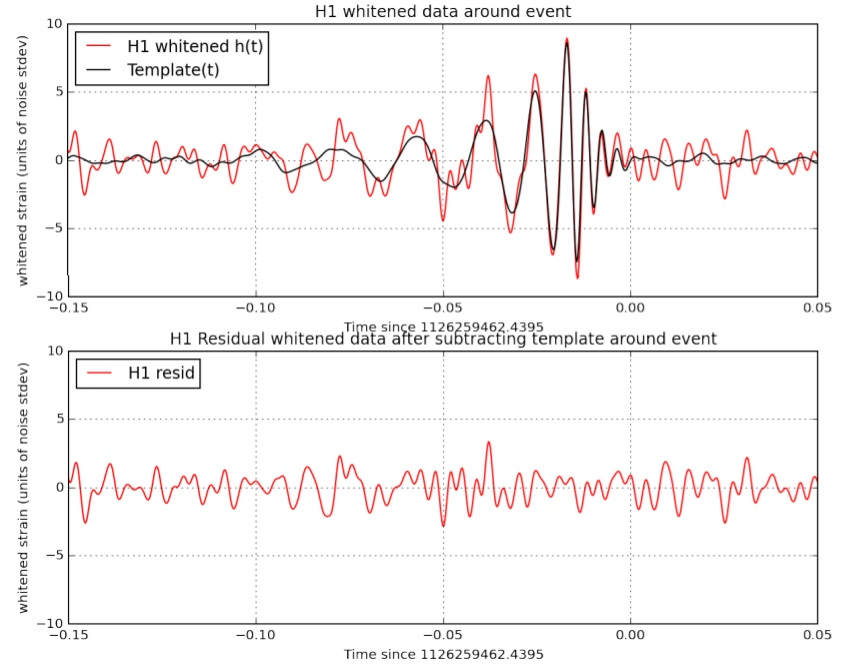
\includegraphics[scale=0.92]{images.tex/template_matching.jpg}
    \caption{Matching the received signal using Gravitational waveform as a template.\\ Source :- \href{https://kiss.caltech.edu/workshops/LISA/presentations/Babak.pdf}{Introduction to Data Analysis of Gravitational Wave Signals by Stanislav Babak}}
\end{figure}

Therefore, we need to apply a “SNR” filter13, taking only the samples above some threshold value of the signal-to-noise ratio. In the LIGO data, it turns out that if one sample has a high SNR, then it is usually surrounded by neighbors that also have high SNR. Most of these are false positives and LIGO performs yet another cut, keeping only the single highest SNR candidate in each such cluster. This further reduces the size of the data set. After that, the software looks for coincidence between the two LIGO antennas. From the reduced data set, a statistic called the log likelihood ratio, or LLR is computed . The larger the LLR for a candidate, the more likely it is to be caused by a signal rather than noise, and vice versa. When a real signal is present in the data, it is generally surrounded by a large number of candidates which are the result of matches by similar-shaped templates to the matching one. This has been determined by many runs in which simulated waveform data have been injected into the data stream to test the software. \\

This allows candidates to be clustered, similar to the way the SNR threshold peaks were clustered; in this case, if a candidate falls within 4 seconds of another candidate that has a higher LLR, the weaker candidate is discarded. It turns out that there is a high probability of finding a low-ranked candidate next to a high ranked one, and so this method successfully trims many low ranked candidates from the sample. However, for candidates with LLR larger than about 6, this clustering method is not effective because the probability of two such candidates being within 4 seconds of one another so low: the recent data run produced one candidate like this about every 5 minutes, or 10, 000 of them for the entire run. The total sample in the data set has now been reduced from 500 million per second to only 10, 000 total, a small enough sample that it is possible to perform detailed statistical testing on each one of them.\\

Once the GW signal is extracted, then it's frequency will be changed by multiplying it with a conversion ratio, such that the resulting frequency lies in the audible range. On September 14 2015, the first characteristic `chirp' sound of the GW150914 was decoded using LIGO. 

\pagbreak


\section{Detection of Gravitational waves using LIGO }
\input{9 Detection_by_ligo.tex/9.1 First Observation}
\subsection{Some Detections of LIGO}

\subsubsection{GW190814}

Two advanced-LIGO detectors (Hanford, Washington and Livingston, Louisiana, USA) and the advanced-Virgo detector (Cascina, Italy), have detected gravitational waves from the inspiral and merger of a stellar-mass black hole and another compact object on 14th August, 2019 at 21:10:39 UTC. It has been named as GW190814 as the date suggests.

\begin{figure}[h]
    \centering
    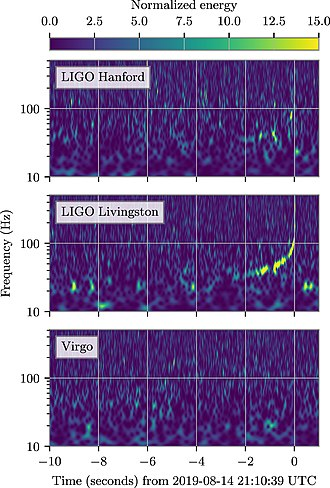
\includegraphics[scale = 0.91]{images.tex/GW190814.jpg}
    \caption{Frequency Vs Time data of GW190814 in three observatories. Source:- \href{https://en.wikipedia.org/wiki/GW190814}{Wikipedia}}
\end{figure}

While the mass of one component of this binary could range from 22.2 to 24.3 $M_\odot$ black hole, the other component which was of 2.6 solar mass could be either a low-mass black hole or a heavy neutron star. The masses of the objects before merging differed by a factor of 9. This makes it the most extreme mass ratio known for some GW event. The source of this GW was in a small patch of sky of around 20 square degrees. Even after doing so much research, the counterpart of the black hole which was in the inspiral mechanism wasn’t observed. It can be that, either black hole consumed the neutron star completely or both were black holes. Had we observe an electromagnetic counterpart, which may not have happened due to a number of reasons, we could say the smaller object is mostly neutron star. 

\pagebreak

\subsection{GW170817}

On 17th August, 2017, LIGO and Virgo detectors observed a gravitational wave named as GW170817. It is known to be produced by two neutron stars merging into each other while spiralling closer and closer. The aftermath of this GW was observed by around 70 observatories on 7 continents as well as through space, across the electromagnetic spectrum, marking a significant breakthrough for multi-messenger astronomy. The discovery and subsequent observations of GW170817 got Breakthrough of the Year award for 2017 by the journal Science.

\begin{figure}[h]
    \centering
    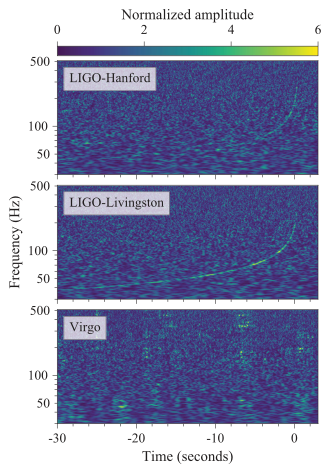
\includegraphics[scale=0.78]{images.tex/GW170817_observatories.png}
    \caption{Frequency Vs Time data of GW170817 in three observatories. Source:- \href{https://en.wikipedia.org/wiki/GW170817}{Wikipedia}}
\end{figure}

The component masses of the binary are inferred to be between 1.17 and 1.60 $M_\odot$. After merging it makes the mass of about 2.74 $M_\odot$. The gravitational wave signal lasted for about 100 seconds. It started with a frequency of 24 $Hz$. It  inspiralled for around 3,000 cycles. The amplitude and frequency increased to a few hundred hertz as both the objects came nearer in the typical inspiral chirp pattern. Lastly, it ended with the collision at 12:41:04.4 UTC which was received as a signal in the interferometer. At first, it arrived at the Virgo detector in Italy. After 22 milliseconds, detectors at the LIGO-Livingston detector in Louisiana, United States got the signals. After another 3 milliseconds, the waves reached at the LIGO-Hanford detector in the state of Washington, United States. It was then compared with a prediction from the general theory of relativity given by Einstein to analyse it further. The source was localised within a sky region of 28\degree square which has a probability of 90\%.

A gamma-ray burst, GRB 170817A was detected. It lasted for $\approx$ 2 seconds. It was detected by Fermi and INTEGRAL spacecrafts. This bursts began at 1.7 seconds after the signal received denoting the merge of the objects. It's a hypothesis that neutron star mergers cause gamma-ray bursts which gets confirmed with this merger.





\pagebreak


\section{Conclusion}
\input{10 Conclusion.tex/10.1 Advancements in Ligo}
\input{10 Conclusion.tex/10.2 Uses in future}
\input{10 Conclusion.tex/10.3 Outcome of paper}

\printbibliography
\end{document}